% -----------------------------------------------
% Template for ISMIR Papers
% 2015 version, based on previous ISMIR templates
% -----------------------------------------------

\documentclass{article}
\usepackage{ismir,amsmath,cite}
\usepackage{graphicx}
\usepackage{color}
\usepackage{booktabs}

% Title.
% ------
\title{Chord Detection Using Deep Learning}


% Single address
% To use with only one author or several with the same address
% ---------------
%\oneauthor
% {Names should be omitted for double-blind reviewing}
% {Affiliations should be omitted for double-blind reviewing}

% Two addresses
% --------------
%\twoauthors
%  {First author} {School \\ Department}
%  {Second author} {Company \\ Address}

% Three addresses
% --------------
\threeauthors
  {First author} {Affiliation1 \\ {\tt author1@ismir.edu}}
  {Second author} {\bf Retain these fake authors in\\\bf submission to preserve the formatting}
  {Third author} {Affiliation3 \\ {\tt author3@ismir.edu}}

% Four addresses
% --------------
%\fourauthors
%  {First author} {Affiliation1 \\ {\tt author1@ismir.edu}}
%  {Second author}{Affiliation2 \\ {\tt author2@ismir.edu}}
%  {Third author} {Affiliation3 \\ {\tt author3@ismir.edu}}
%  {Fourth author} {Affiliation4 \\ {\tt author4@ismir.edu}}

\begin{document}
%
\maketitle
%
\begin{abstract}
In this paper, we utilize deep learning to learn high-level features for audio chord detection. The learned features, obtained with a deep neural network in bottleneck architecture, give promising results and outperform state-of-the-art systems. We present and evaluate the results for various methods and configurations, including input pre-processing, a bottleneck architecture, unsupervised pre-training, and SVMs vs.\ HMMs. 
\end{abstract}
%
\section{Introduction}
The goal of automatic chord detection is to automatically recognize the chord progression in a music recording. It is an important task in the analysis of western music and music transcription, and it can contribute to applications such as music similarity measures, key detection, structural segmentation, and other semantic analysis tasks. Despite early successes in chord detection by using pitch chroma features and Hidden Markov Models (HMMs) \cite{fujishima1999realtime}, recent attempts at improving detection accuracy are only met with moderate success \cite{}.\footnote{insert references here!} 

In recent years, deep learning approaches have gained significant interest in the machine learning community as a way of building hierarchical representations from large amounts of data. Deep learning has been applied successfully in many fields. For instance, a system for speech recognition with deep learning was able to outperform state-of-the-art systems (not using deep learning) \cite{hinton2012deep}. Several studies indicate that deep learning methods can be very successful when applied to Music Information Retrieval (MIR) tasks, especially when used for feature learning \cite{lee2009unsupervised,battenberg2012analyzing,humphrey2012moving,hamel2010learning}. Deep learning, with its potential to untangle complicated patterns in large amounts of data, should be well suited for the task of chord detection.

In this work, we investigate Deep Neural Networks (DNNs) for learning high-level and more representative features in the context of chord detection, effectively replacing the widely used pitch chroma intermediate representation. 
We present individual results for different pre-processing options such as time splicing and filtering (see Sect.~\ref{sec:pre-proc}), training scenarios (see Sect.~\ref{sec:train}), architectures (see Sect.~\ref{sec:arch}), and output classifiers (see Sect.~\ref{sec:class}).\footnote{check section references!} %Since chords last for a period of time instead of static and instantaneous, we apply time splicing and convolution to account for relations between nearby frames. Then we can derive transition probability between chords from our training set and use the high-level probabilistic features as emission probability to decode the whole chord sequence. Alternatively we also train SVMs with same features and do the static classification frame by frame.

%The definition of chords is, simply speaking, \"simultaneous sounding of two or notes". But in reality this is not the case. Real music often generate not only chord tones but nonchord tones with no guarantee of simultaneity. To make it more complicated, sometimes either some notes are missing or more notes are added-on into a chord. Thus, traditional chord detection systems exhibit a set of practical difficulties. Deep learning has a great potential in entangling complicated patterns within large data. Therefore, although chord detection is one of the most difficult and challenging tasks for music analysis, applying deep learning methods is much potentially promising. 
%

%\begin{figure}
% \centerline{\framebox{
% 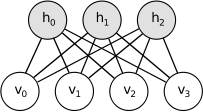
\includegraphics[width=\columnwidth]{rbm.png}}}
% \caption{DBN with one visible layer and one hidden layer}
% %\label{fig:example}
%\end{figure}

\section{related work}
During the past decade, deep learning has been considered by the machine learning community to be one of the most interesting and intriguing research topics. Deep architectures promise to remove the necessity of custom-designed and manually selected features as neural networks should be more powerful in disentangling interacting factors and thus be able to create meaningful high-level representations of the input data. Generally speaking, deep learning combines deep neural networks with an unsupervised learning model. Two major learning models are widely used for this purpose: Restricted Boltzmann Machines (RBMs) and Sparse Auto Encoders. A deep architecture comprises multiple stacked layers based on one of these two models. These layers can be trained one by one, a process that is referred to as ``pre-training'' the network. In this work, we employ RBMs to pre-train the deep architecture in an unsupervised fashion; this is called a Deep Belief Network (DBN). DBNs, composed of a stack of RBMs, essentially share the same topology with general neural networks: DBNs are generative probabilistic models with one visible layer and several hidden layers.\footnote{shouldn't there be any general references in this whole paragraph?}
 
Since Hinton proposed a fast learning algorithm for DBNs \cite{hinton2006fast}, they have been widely used for initializing deep neural networks. In deep structures, each layer learns relationships between units in lower layers. With the number of RBM layers increasing the complexity of the system increases, making the structure, theoretically, more powerful. An extra soft max output layer can be added to the top of the network; its output can be interpreted as the likelihood of each class.

LeCun formulated the idea of applying the Convolutional Neural Networks (CNNs) to images as well as speech and other time-series signals \cite{lecun1995convolutional}. This approach, shown in Fig.~\ref{fig:cnn}, allows to deal with the variability in time and space to a certain degree; furthermore, it reduces the overfitting problem BY DOING THIS AND THAT\footnote{explain me!}. CNNs can be seen as a special kind of neural network in which the weights are shared across the input within a certain spatial or temporal area. The weights thus act as a kernel filter applied to the input. CNNs have been particularly successful in image analysis. For example, Norouzi et al.\ used Convolutional RBMs to learn shift-invariant features \cite{norouzi2009stacks}. 
\begin{figure}
 \centerline{\framebox{
 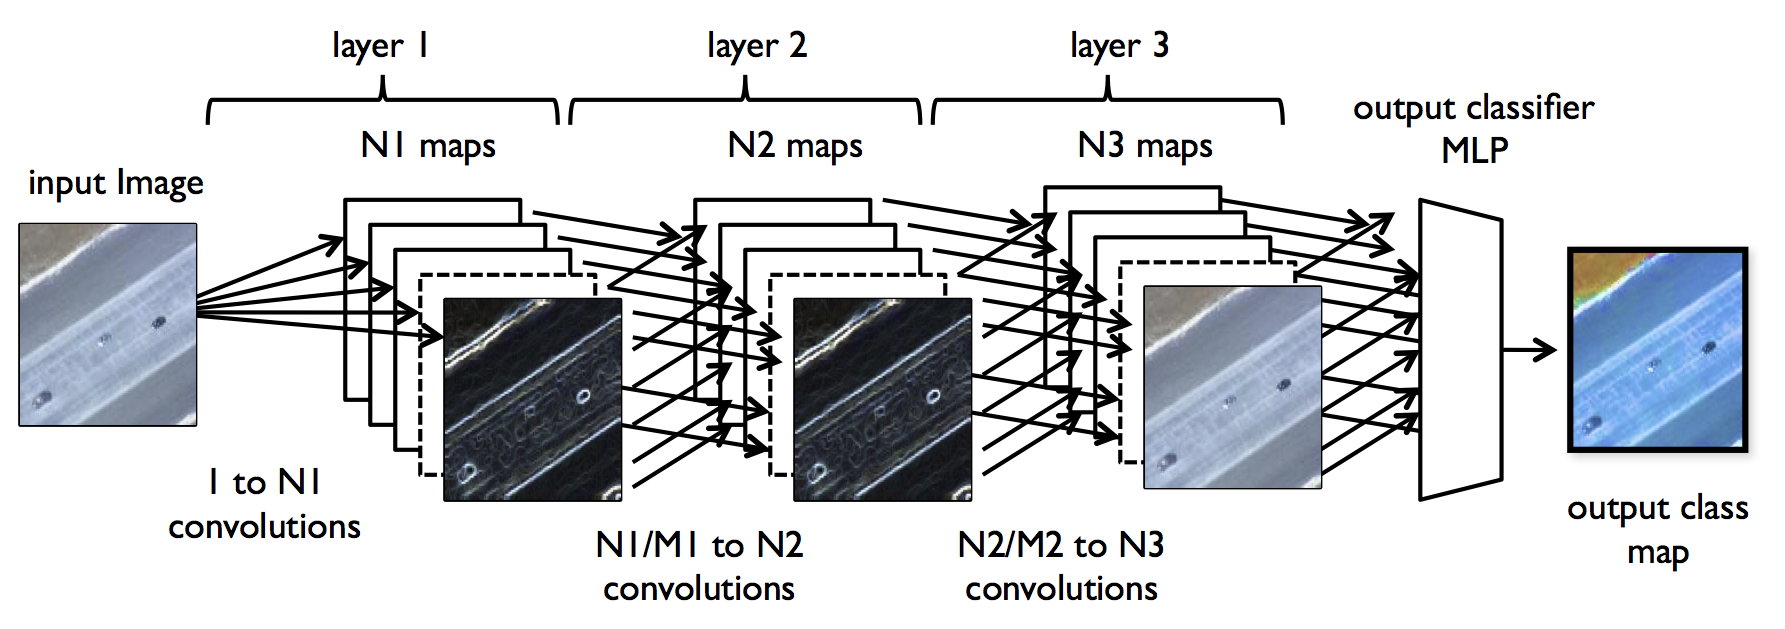
\includegraphics[width=\columnwidth]{neuralnet.png}}}
 \caption{CNNs used for image classification}
 \label{fig:cnn}
\end{figure}
Modifications of the network architecture obviously result in different results. Grezl et al.\ used a so-called bottleneck architecture neural network to obtain features for speech recognition and showed that these features improve the accuracy of the task \cite{grezl2007probabilistic}. The principle behind the bottleneck-shaped architecture is that the number of neurons in the middle layer is lower than in the other layers as shown in Fig.~\ref{fig:bottleneck}.

Recently, more researchers investigated deep learning in the context of MIR. Lee et al.\ pioneered the application of convolutional deep learning for audio feature learning \cite{lee2009unsupervised}. Hamel et al.\ used the features learned from music with a DBN for both music genre classification and music auto-tagging \cite{hamel2010learning}; their system was successful in MIREX 2011 with top-ranked results. Battenberg employed a conditional DBN to analyze drum patterns \cite{battenberg2012analyzing}. The use of deep architectures for chord detections, however, has not yet been explored, although modern neural networks have been employed in this field. For instance, Boulanger et al.\ investigated recurrent neural networks \cite{boulanger2013audio} and Humphrey has explored CNNs \cite{humphrey2012rethinking,humphrey2012learning}. While they also used the concept of pre-training, their architectures have only two or 3 layers and thus cannot be called ``deep''.
\begin{figure}
 \centerline{\framebox{
 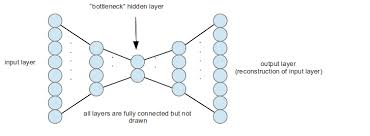
\includegraphics[width=\columnwidth]{bottleneck.jpeg}}}
 \caption{Bottleneck Neural Network Architecture}
 \label{fig:bottleneck}
\end{figure}

The basic buildings blocks of most modern approaches to chord detection can be traced back to two influential publications: Kawakami proposed to use HMMs for representing chords as hidden states and to model the transition probability of chords \cite{kawakami2000hidden} and Fujishima introduced pitch chroma vectors extracted from the audio as input feature for chord detection \cite{fujishima1999realtime}. Since then there have been a lot of studies using chroma features and HMMs for chord detection\footnote{cite: H. Papadopoulos and G. Peeters, Large-scale study of chord estimation algorithms based on chroma representation and hmm, Cho et al. EXPLORING COMMON VARIATIONS IN STATE OF THE ART CHORD RECOGNITION SYSTEMS}. Examples for recent systems are  Ni, using genre-independent chord estimation method based on HMM and chroma features \cite{ni2012using} and Cho used multi-band features and a multi-stream HMM for chord recognition \cite{cho2013mirex}. Training HMMs with pitch chroma features arguably is the standard approach for this task and the progress is less marked by major innovations but by optimizing and tuning specific components. 

%In this work, we employ deep learning to come up with a novel system for chord detection. 

%\begin{figure}
% \centerline{\framebox{
% \includegraphics[width=\columnwidth]{1.png}}}
% \caption{Underlying chord states from melody}
% %\label{fig:example}
%\end{figure}

\section{DBN-DNN}
\subsection{Input Representations}
Constant Q transform (CQT) is perceptually inspired time-frequency transformation for audio, where the window length of discrete fourier transform has a fixed ratio with the ``pitch". CQT can retain mostly all the pitch information as well as lower the dimension of inputs. Audio files are first downsampled to 11025Hz. We implemented CQT as a filterbank of Gabor filters, spaced at 36 bins per octave, ie. 3 bins per semitone, yielding 180 bins spanning from 110 Hz to 3520 Hz. We apply PCA to reduce the redundant dimension as well as to decorrelate each dimension, and apply Z-Score normalization\cite{sola1997importance}. 

\subsection{Pre-Processing}\label{sec:pre-proc}
Since chords are dynamic signals changing along with the time, and the current state has relationship between both previous states and future states. In order to extract these relations and information within temporal neighbors, we apply several pre-processing approaches to the input representation. 
\subsubsection{Time Splicing}
Time splicing is to splice the current frame with a few frames on both side, yielding a larger frame as shown in figure 3. For example, in the figure, assuming there are 7 frames in a piece. If we apply 1 time splicing, which means we splice the current frame with previous 1 frame and next 1 frame together. For 4th frame, we group 3rd, 4th and 5th frame and splice them into one bigger frame, which is the new representation for the 4th frame, the same operation will be applied on the 5th frame. Therefore there will be some overlap between neighboring frames. We conduct such operation along over all frames in each piece with different splice amount. 
\begin{figure}
 \centerline{\framebox{
 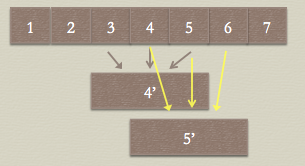
\includegraphics[width=\columnwidth]{timesplice}}}
 \caption{Illustration for time splicing}
 %\label{fig:example}
\end{figure}

\subsubsection{Convolution}
Though we don't use CNNs, we employ the similar idea as CNNs. Essentially CNNs are automatically add one or several convolutional layers at the beginning of neural networks. The convolutional layer can be interpreted as a linear filter that conduct a convolution on the input signal plus a non-linear transformation, sometimes combined with pooling operation as well, as in \eqnref{Covulution}.
\begin{equation}\label{Covulution}
Y = pool(sigm(K \ast X + B))
\end{equation}  
Where $Y$ is the output of a convolutional layer, $K$ is the linear kernel filter, $X$ is the input, $B$ is the bias, $sigm()$ is a non-linear transform, $pool()$ is a down-sampling operation. The core transformation is the $\ast$ operation, which is to do the convolution operation between filters and input representation. 
Instead of training the filters automatically, we can make use of the prior knowledge to design the filters manually. In the case of chord detection, given we mainly want to extract time information by convolution, so we design time domain filters. \\
The first type of our filter is low pass filter. We employ a simple single pole low pass filter due to its easy parameter configuration. Given that our system is not designed for real-time processing, we can use the ``filtfilt" techniques to ensure the filter has linear phase response. A ``filtfilt" filter is centered around the current frame in time domain. \\
Under the assumption that the frame that is located in the middle of a chord is way more obvious and easier to be detected than the frame that is located at the boundary of a chord, we also design another two types of filters, both of which have exponential decay shaped impulse response, the different equation as in \eqnref{filter1} \eqnref{filter2}. 
\begin{equation}\label{filter1}
y_{1}(n) = \sum_{k=1}^N a^{-k+1} x(n-N+k)
\end{equation}
\begin{equation}\label{filter2}
y_{2}(n) = \sum_{k=1}^N a^{-k+1} x(n+N-k)
\end{equation} 
Where $a$ is the exponential base, $N$ is the filter length. 
These filters are not centered around the current frame anymore, but shifted to either side. Their impulse response are symmetric, one is to take past frames into consideration, while the other is to take next frames into consideration. We call these filters as ``extension filters".  \\
In a further processing, we combine the ideas of time splicing and convolution: we either conduct time splicing on the output of the low pass filter, or splice the output of different filters together, as in figure 4.
\begin{figure}
 \centerline{\framebox{
 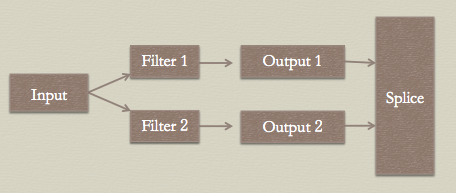
\includegraphics[width=\columnwidth]{CNN}}}
 \caption{Splicing output of different filters}
 %\label{fig:example}
\end{figure}
We call this kind of processing as ``splice filtering. 
 
\subsection{DBN}\label{sec:train}
Due to the deep structure, deep neural networks are impractically trained directly by back propagation using gradient decent. Therefore a pre-train processing under an unsupervised training is applied for better initialize the networks. As mentioned before, we employ RBMs to build up DBNs for this purpose. 
In training RBMs using Gibbs sampling algorithms, the objective is to remain as much information as possible between output and input. The computation between layers can represented as:
 \begin{equation}\label{dbn}
Y_{l} = sigm(W_{l}X_{l} + B_{l})
\end{equation}  
Which can be exactly the same as neural networks. Therefore, we can fine-tune the networks in a supervised manner using standard back propagation with respect to some loss criterion. We use cross-entropy loss function in this work.  

\subsection{Architecture}\label{sec:arch}
We build a 6 layer deep networks in this work and compare the bottleneck architecture and the common architecture, in which all layers share the same amount of neurons. In the common architecture, each layer has 1024 neurons; in the bottleneck architecture, the middle layer has 256 neurons, the layers besides middle layer have 512 neurons and the rest layers have 1024 neurons. At last, a soft-max output layer is stacked on top of the 6 layer networks, as in \eqnref{softmax}.
\begin{equation}\label{softmax}
software(Y_{l}) = \frac{exp(Y_{l})}{\sum_{k=1}^N exp(Y_{k})}
\end{equation}
The DBN-DNN system is implemented using the Kaldi package developed by John Hopkins University \cite{povey2011kaldi}.
 
\section{Post-classifiers}\label{sec:class}
Although we can interpret the output of softmax layer as likelihood of each class and take the maximum directly to make the final decision, we can also treat the output as the intermediate features and train other classifiers based on these features to make the final decision. 
\subsection{HMMs}
Traditionally speaking, chord detection can be treated as a task to estimate underlying hidden chord states from a complex mixture, a task which HMMs is well suited. In HMM-based chord detection systems, feature vectors are extracted from audio signals as the observations, and chords are interpreted as hidden states. The most widely used input features for HMMs are chroma-based features. Some modified HMMs such as ergodic HMMs and key-independent HMMs have been also explored. In this work, a simple first-order HMM is applied. Given the probabilistic property of softmax layer output, we can use them directly as emission probabilities in the context of HMMs. Therefore, we do not have to train HMMs using commonly used Baum-Welch algorithm. Instead, we count the histogram of each class in our training set to be initial probabilities, and use bigram of chord transitions to calculated the transition probabilities. Finally, we employ the Viterbi decoding algorithm to find the global optimal state sequence, which is the final prediction of the chords. 
\subsection{Support Vector Machines}
Alternatively, we can use static classifiers as well. Because of general good performance, Support Vector Machines (SVMs) are chosen in this work. We train a SVM using the features learned by DBN-DNN, and do the classification for every frame for the test samples followed by a simple prediction smoothing. 

\section{Evaluation Metric}
We use the same evaluation metric as MIREX 2013 in the audio chord detection task. Chord symbol recall (CSR) and weighted chord symbol recall (WCSR) are used to estimate how well the predicted chords match the ground truth. CSR is defined as the total duration of segments where the predictions match the ground truth divided bythe total duration of the song, formulated as in \eqnref{csr}. WCSR is to weight CSR with the songs' length.  
\begin{equation}\label{csr}
CSR = \frac{1}{n} \sum_{k=1}^n \frac{C_{k}}{N_{k}}
\end{equation}
Where $n$ is the number of test samples, $C_{k}$ is the number of frames that are correctly detected in kth test sample, $N_{k}$ is the total frames in kth test sample. 

\section{Experiment}
\subsection{Data Preparation}
Our dataset is collected from a variety of different sources, yielding a 311-piece collection. The data is composed of 180 songs from Christopher Harte's Beatles dataset, 100 songs from the RWC Pop dataset, 18 songs from the Zwielicht dataset and 13 songs from Queen dataset. Each song is mixed to monaural and down-sampled to 11025 Hz. Ground truth time-aligned chord symbols are mapped to the major/minor dictionaries comprising 25 chord labels:
\begin{equation}
C_{majmin} \subset {N} \cup S \times {maj,min}
\end{equation}
Where S represents 12 pitch classed and N is the unknown chord label, yielding totally 25 chord classes. Evaluation is based on WCSR, which is proposed in the previous section. Since we only map the ground truth into major and minor scale, we consider the chords other than triad major, triad minor, seventh major, seventh minor to be N chords. For instance, G:maj and G:maj7 are all mapped to `Gmaj'; G:dim and G:6 are all mapped to `N'. 
\subsection{DBNs vs. DNNs}
There are three scenarios for training: only training DBNs; only training DNNs; and combined DBNs and DNNs. For comparison, we do not apply any pre-processing to the input data, ie. the input data is the audio CQT followed by PCA. In DBNs scenario, since it is a pure unsupervised training, we take the output of bottleneck layer as output, and use SVMs as post classifiers. Whereas we train the networks in a pure supervised manner in DNNs scenario, in which we directly use back propagation to train the neural networks. Viterbi decoding is used for post processing. In the last case of DBN-DNN, we firstly employ RBMs to build up DBNs, and use it as the initial configuration of DNNs followed by back propagation. Both SVMs and HMMs are applied. In all cases, bottleneck architecture is in use. The results are listed in table 1. 

\begin{table}[h]
\begin{tabular}{|c|c|c|}
\hline
Training Strategy & Post-classifier & WCSR  \\ \hline
DBNs              & SVMs            & 0.141 \\ \hline
DNNs              & HMMs            & 0.159      \\ \hline
DBN-DNNs          & SVMs            & 0.645 \\ \hline
DBN-DNNs          & HMMs            & 0.755 \\ \hline
\end{tabular}
\caption{Chord detection performance of DBNs vs. DNNs}
\end{table}

\subsection{Common Architecture Vs. Bottleneck Architecture}
As mentioned before, we employ a bottleneck architecture in this work. According to \cite{grezl2007probabilistic}, deep networks are suitable in a bottleneck architecture to learn high-level features. We can consider the bottleneck networks as two halves. The first half is from the first layer to the bottleneck layer, in which the number of neurons gradually decreases. This is actually an encoding or compression process. The useful information gets compacter as well as the redundant information can be gotten rid of. The second half is from the bottleneck layer to the last layer, in which the number of neurons gradually increases. We can see it as a decoding process. By these two processes, the networks are able to extract the useful information and discard the redundant ones. Another benefit of bottleneck architecture is that it can reduce the overfitting issue by decreasing the complexity of the system. We compare the common architecture and the bottleneck architecture under the same configurations. In comparison, the configurations are: HMMs as post-classifiers; DBN-DNNs as training strategy. The results are listed in table 2.

% Please add the following required packages to your document preamble:
% \usepackage{booktabs}
\begin{table}[h]
\begin{tabular}{@{}cccc@{}}
\toprule
Architecture                   & Pre-processing                      & \begin{tabular}[c]{@{}c@{}}Training\\ WCSR\end{tabular} & WCSR  \\ \midrule
Common                         & None                                & 0.843                                                      & 0.703 \\
Bottleneck                     & None                                & 0.855                                                      & 0.755 \\
Common                         & 2 Time Splicing                     & 0.903                                                  & 0.712 \\
\multicolumn{1}{l}{Bottleneck} & \multicolumn{1}{l}{2 Time Splicing} & 0.892                                 & 0.821 \\ 
Common     & Splice Filtering & 0.985 & 0.876 \\
Bottleneck & Splice Filtering & 0.936 & 0.919 \\ \bottomrule
\end{tabular}
\caption{Chord detection performance of different architecture}
\end{table}

\subsection{Filters Evaluation}
As stated in previous section, we investigate to design different filters in pre-processing. The first type is linear phase signal pole filter, the difference equation is formulate as \eqnref{IIR}:
\begin{equation}\label{IIR}
y_{n} = (1-\alpha) y_{n-1} + \alpha x_{n}
\end{equation}
Normally, the IIR filters do not have a linear phase response. But we use filtfilt technique to achieve zero phase. Noting that there is only one parameter $\alpha$ which determines the frequency response shape. We conduct a grid search for this parameter, starting from 0.25 to 0.75 with the step size of 0.25. Meanwhile we compare it with different five-order FIR low-pass filter centered around the current frame. The FIR coefficients are exponentially decreased in both side, ie. the impulse response is in Laplace shape. Furthermore, we also combine the ideas of convolution and time splicing. We concatenate the output of low-pass filter together as time splicing does. Inspired by CNNs, we can also concatenate the output of different filters, the results are shown in figure 5.

\begin{figure}
 \centerline{\framebox{
 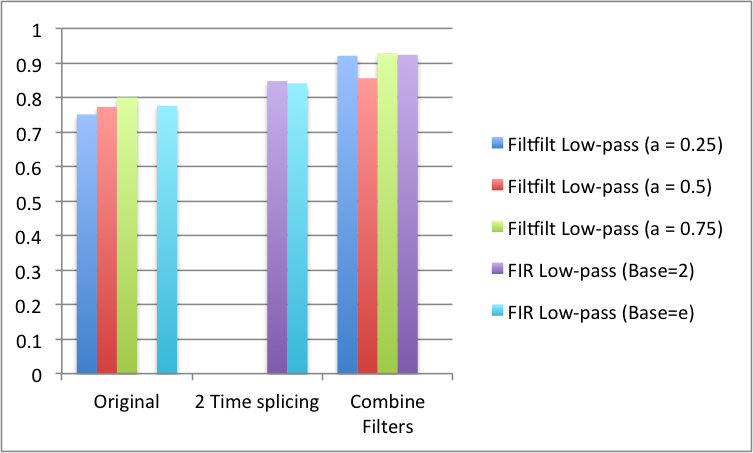
\includegraphics[width=\columnwidth]{filters.png}}}
 \caption{Comparison Between different filters}
 %\label{fig:example}
\end{figure}

\subsection{Learning Chords Vs. Learning Pitches}
Because of the hierarchical property of chords, our learning targets are not limited to chords themselves. Since chords can be decomposed into pitches, therefore we could let the networks learn pitch information instead of chords. By doing so, we hope it can decrease the abstraction and complexity of the task. The main reason for that is pitches are more directly related to the input representations, ie. CQT. It will, however, lead to another issue which is we will transfer the single target learning task to multi-target learning. We use several settings based on the previous experiments to conduct the comparison between chords and pitches. The results are listed in table 4. 

\begin{table}[h]
\begin{tabular}{@{}cccc@{}}
\toprule
Learning Targets & Pre-processing   & \begin{tabular}[c]{@{}c@{}}Post-\\ processing\end{tabular} & WCSR  \\ \midrule
25 Chord Classes & Splice Filtering & Viterbi                                                    & 0.919 \\
12 Pitch Classes & Splice Filtering & HMMs                                                       & 0.78  \\ \bottomrule
\end{tabular}
\caption{Chord detection performance of different learning targets}
\end{table}
As seen from the results, learning pitches does not really work. There should be several potential reasons. Even though we believe the idea of decomposing chords will bring some benefits, some practical issue may impact such benefits: firstly, multi-target learning is relatively more difficult for the model per se to train. Since in our implementation of multi-target training, we assign each target a equal posterior, which is less obvious than the single target for models to learn. Second, in the real audio files, some notes are occasionally removed from or added into a chord, which could make the pitch ground truth inaccurate. Therefore, we give up this idea in our final evaluation. 

\section{Results and Discussion}
\subsection{Results}
From previous discussions and comparisons, several settings show the most promise. So we decide to use them as the default configuration in our final evaluations: bottleneck structure outperforms the common structure both in accuracy and time-complexity; DBN-DNNs training strategy beats DBNs and DNNs training strategies without much surprise; splice filtering similar to what CNNs do, generally speaking, yields a better result than the others; finally, Viterbi decoding as post classifiers are more appropriate for this task due to the dynamic properties of chords.  \\
In previous published results \cite{cho2011feature} on the similar dataset is around 80\%. We present the mean accuracy of 3 fold cross-validation obtained on our 311-piece dataset at the major/minor level (total 25 classes). We compare our results with Chordino approach on our dataset, though in an unfair way, as baseline system. Noting that Chordino system can not only detect major/minor scale, it can detect as much as 120 different chords. Thus we map the Chordino results into our major/minor scale. In this mapping, due to the different chord annotation rules, we could make mistakes through imperfect parsing. The results are listed in table 4, in which Type1 pre-processing is to splice the 5-order FIR low-pass filter and extension filters; whereas Type2 pre-processing is to splice the single-pole IIR low-pass filter and extension filters. 

% Please add the following required packages to your document preamble:
% \usepackage{booktabs}
\begin{table}[h]
\begin{tabular}{@{}ccc@{}}
\toprule
Methods   & Pre-processing & WCSR   \\ \midrule
Chordino & N/A            & 0.625       \\
Proposed DBN-DNNs & Type1          & 0.911 \\
Proposed DBN-DNNs & Type2          & 0.919   \\ \bottomrule
\end{tabular}
\caption{Chord detection performance of different methods}
\end{table}

\subsection{Discussion}
We presented a comprehensive system for chord detection, that is competitive with the existing start-of-the-art systems. Our DBN-DNNs model can learn a high-level probabilistic representations for chords. The Viterbi algorithm is applied to find a global optimal path based on the output of our DBN-DNNs as the predicted chord sequence. Furthermore, the bottleneck structure have a stronger learning ability for chords information than the common architecture. By the process of ``encoding" and ``decoding", the networks retain the ``essential information" but discard the redundant ones. The results also indicate that applying pre-processing will significantly increase the accuracy. That's because it will introduce temporal continuity and dynamics into feature representation. Intuitively, dynamic programming algorithms such as Viterbi decoding outperforms the static classifiers such as SVMs due to the dynamic property of chords. Therefore introducing transition probability makes more sense. 



\bibliography{ISMIR2015template}
\end{document}
